\documentclass{article}
\usepackage{algorithm}
\usepackage{amsmath}
\usepackage{algpseudocode}
\usepackage[utf8]{inputenc}
\usepackage{graphicx}
\newtheorem{definizione}{Definizione}
\newtheorem{theorem}{Teorema}
\newtheorem{corollary}{Corollario}
\title{Introduzione all'Intelligenza Artificiale 2022}
\author{Ambra Manattini}
\date{February 2022}

\begin{document}

\maketitle

\section{Agenti Intelligenti}
Primo obiettivo: agenti per la risoluzione di problemi vista come ricerca in uno spazio di stati (\textbf{problem solving})

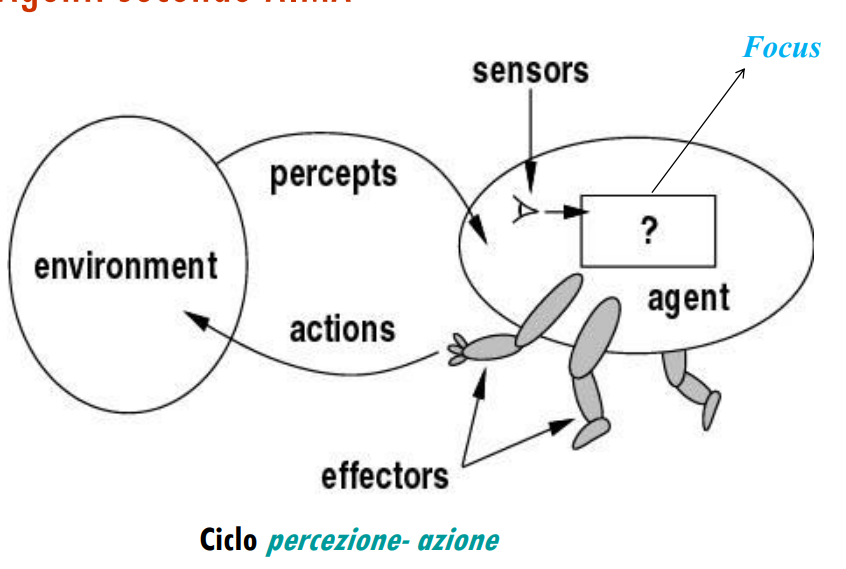
\includegraphics[width=\linewidth]{1.png}

L'agente esegue il ciclo percezione-azione. Il focus è il programma dell'agente

\subsection{Caratteristiche degli agenti}
\begin{itemize}
    \item \textbf{Situati}: ricevono percezioni dall'ambiente e agiscono mediante \textit{azioni}
    \item \textbf{Abilità sociale}: capaci di comunicare, collaborare, difendersi da altri agenti
    \item Hanno \textbf{credenze, obiettivi, intenzioni}
    \item \textbf{Embodied}: hanno un corpo fisico, fino a considerare i meccanismi delle emozioni
\end{itemize}

La scelta dell'agente è una funzione della \textbf{sequenza percettiva}, definisce l'azione da compiere in base a ogni sequenza percettiva, implementata da un programma agente
\begin{figure}
    \centering
    
\includegraphics[width = \linewidth]{2.png}
    \caption{funzione agente: definisce l'azione da compiere per ogni sequenza percettiva}
    \label{fig:my_label}
\end{figure}


\subsection{Agenti Razionali}
Un agente razionale interagisce col suo ambiente in maniera efficace, perché serve un \textit{criterio di valutazione} oggettivo dell'effetto delle azione dell'agente (es costo minimo di un cammino alla soluzione)


\textbf{Valutazione della prestazione}

Misura di prestazione
\begin{itemize}
    \item Esterna (come vogliamo che il mondo evolva)
    \item Scelta dal progettista a seconda del problema
    \item Possibilmente valutata su ambienti diversi
\end{itemize}
La razionalità dipende da
\begin{itemize}
    \item Misura di prestazione
    \item Conoscenza pregressa dell'ambiente
    \item Percezioni presenti e passate
    \item Capacità dell'agente
\end{itemize}
Un \textbf{agente razionale} per ogni sequenza di percezioni compie l'azione che massimizza il valore atteso della misura delle prestazioni, considerando le sue percezioni passate e la sua conoscenza pregressa.

Non è perfetto e non conosce il futuro, potrebbero essere necessarie azioni di acquisizione di informazioni o esplorative. Le capacità dell'agente sono limitate.
Raramente tutta la conoscenza dell'ambiente può essere fornita a priori, l'agente razionale deve essere in grado di modificare il suo comportamento con l'esperienza (\textit{si adatta})

\par \textbf{Agente autonomo}

È autonomo nella misura in cui il suo comportamento dipende dalla sua capacità di ottenere esperienza

\subsection{Ambienti}
Definire un problema per un agente significa caratterizzare l'ambiente in cui l'agente opera (\textit{ambiente operativo}
\subsubsection{PEAS}
Descrizione PEAS dei problemi
\begin{itemize}
    \item \textbf{P}erformance | prestazione
    \item \textbf{E}nvironment | ambiente
    \item \textbf{A}ctuators | attuatori
    \item \textbf{S}ensors | sensori
\end{itemize}
\begin{figure}
    \centering
    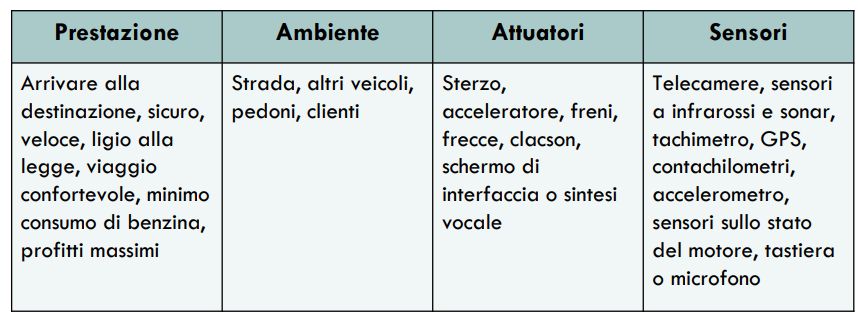
\includegraphics[width=\linewidth]{8.png}
    \caption{es. agente guidatore di taxi}
\end{figure}

\subsection{Osservabilità}
\begin{itemize}
    \item Completamente osservabile: l'apparato percettivo è in grado di dare una consocenza completa dell'ambiente o almeno tutto quello che serve a decidere l'azione, non c'è bisogno di mantenere uno stato del mondo esterno
    \item Parzialmente osservabile: sono presenti limiti o inaccuratezza dell'apparato sensoriale
\end{itemize}
\subsubsection{Ambiente singolo/multi agente}
\begin{itemize}
    \item Agente/non agente: il mondo può cambiare per eventi, non necessariamente per azioni di agenti
    \item Multi agente competitivo (scacchi)
    \item Multi agente cooperativo: comunicazione, stesso obiettivo
\end{itemize}
\subsubsection{Predicibilità}
\begin{itemize}
    \item Deterministico: stato successivo completamente determinato dallo stato corrente dell'azione
    \item Stocastico: esistono elementi di incertezza con associata probabilità
    \item Non deterministico: si tiene traccia di più stati possibili risultato dell'azione
\end{itemize}
\subsubsection{Episodico/sequenziale}
\begin{itemize}
    \item Episodico: l'esperienza dell'agente è divisa in episodi atomici indipendenti
    \item Sequenziale: ogni decisione influenza le successive
\end{itemize}
\subsubsection{Statico/dinamico}
\begin{itemize}
    \item Statico: il mondo non cambia mentre l'agente decide l'azione
    \item Dinamico: cambia nel tempo, va osservata la contingenza
    \item Semi dinamico: l'ambiente non cambia, ma la valutazione dell'agente sì
\end{itemize}
\subsubsection{Discreto/continuo}
\begin{itemize}
    \item Possono assumere valori discreti o continui:
    \begin{itemize}
        \item Lo stato
        \item Il tempo
        \item Le percezioni
        \item Le azioni
    \end{itemize}
    \item Combinatoriale vs infinito
\end{itemize}
\subsubsection{Noto/ignoto}
\par Si riferisce allo stato di conoscenza dell'agente sulle leggi fisiche dell'ambiente; se l'agente conosce l'ambiente o deve compiere azioni esplorative.

Noto != Osservabile

\subsection{Struttura di un agente}
Un agente è formato da \textit{architettura} e \textit{programma}. 
Il programma dell'agente implementa la funzione \(Ag: P \rightarrow Az\) 
\begin{enumerate}
    \item Prende in input delle percezioni e ritorna delle azioni
    \item Aggiorna la memoria in base alle percezioni
    \item Sceglie la migliore azione possibile in base alla memoria
    \item Aggiorna la memoria a seconda dell'azione che abbiamo fatto
\end{enumerate}
\subsubsection{Agente basato su tabella}
La scelta dell'azione è un accesso a una \textit{"tabella"} che associa un'azione a ogni possibile sequenza di percezioni. L'implementazione tramite actual tabella è ingestibile per vari motivi

\subsection{Agenti reattivi semplici}

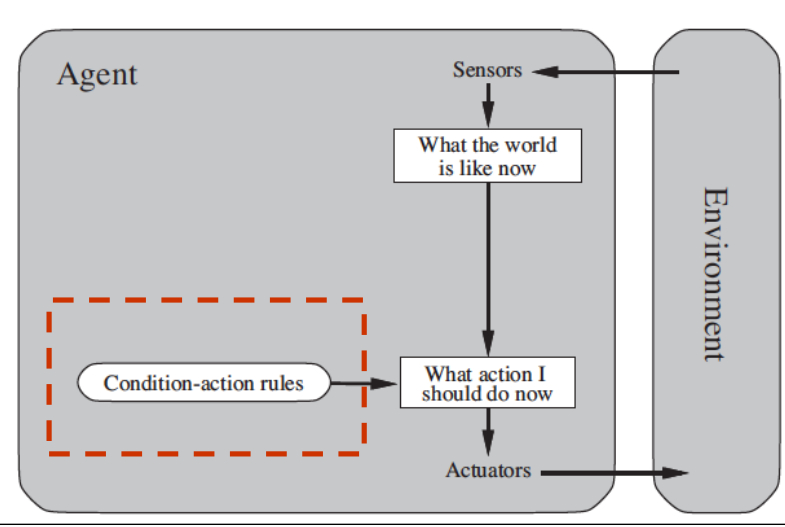
\includegraphics[width = \linewidth]{3.png}

Non c'è storia in memoria, non tiene conto delle cose precedenti.

\begin{math}
\textbf{function} Agente-Reattivo-Semplice (percezione)
\\ \textbf{returns}\,azione
\\ \textbf{persistent}: regole,\, un\, insieme\,di\,regole\, \textit{condizione-azione (if-then)}
\\ stato \leftarrow Interpreta-Input(\textit{percezione})
\\ regola \leftarrow Regola-Corrispondente(\textit{stato, regole})
\\ azione \leftarrow regola.Azione
\\ \textbf{return}\,azione
\end{math}

\subsection{Agenti basati su modello}
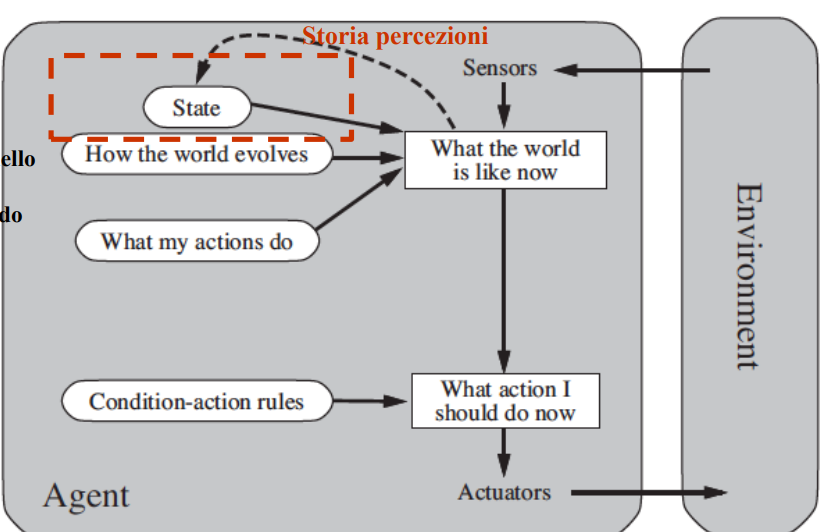
\includegraphics[width=\linewidth]{4.png}
\textbf{Si introduce uno stato storia delle percezioni, abbiamo di nuoco lo stato e il modello del mondo}

\begin{math}
\textbf{function}\, Agente-Basato-su-Modello\,(percezione)
\\\textbf{return}\, azione
\\\textbf{persistent:}\,\textit{stato},\,una\,descrizione\,dello\,stato\,corrente
\newline\null\qquad\textit{modello},\,conoscenza\,del\,mondo
\newline\null\qquad\textit{regole},\,un\,insieme\,di\,regole\,condizione-azione
\newline\null\qquad\textit{azione},\,l'azione\,piu'\,recente
\\\textit{stato}\leftarrow Aggiorna-Stato(stato,azione,percez.,modello)
\\\textit{regola}\leftarrow Regola-Corrispondente(stato,regole)
\\\textit{azione} \leftarrow regola.Azione
\\\textbf{return}\,azione
\end{math}

Lo stato si aggiorna in base alla sequenza di azioni fatte e il modello del mondo.
\subsection{Agente con obiettivo}

\par Guidati da un obiettivo nella celta dell'azione, l'azione migliore dipende dall'obiettivo che devo raggiungere, devo pianificare una sequenza di azioni per raggiungere questo obiettivo.

Meno efficienti ma più flessibili (può cambiare l'obiettivo)

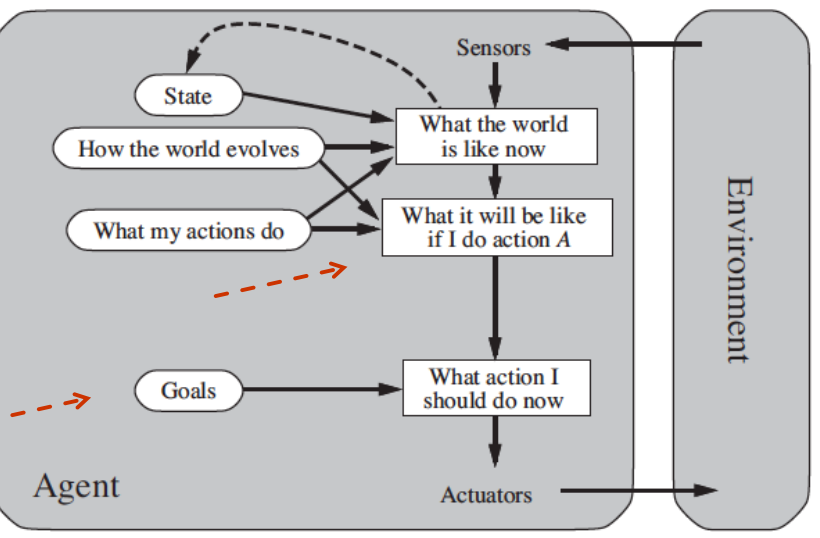
\includegraphics[width=\linewidth]{5.png}

\subsection{Agenti con valutazione di utilità}

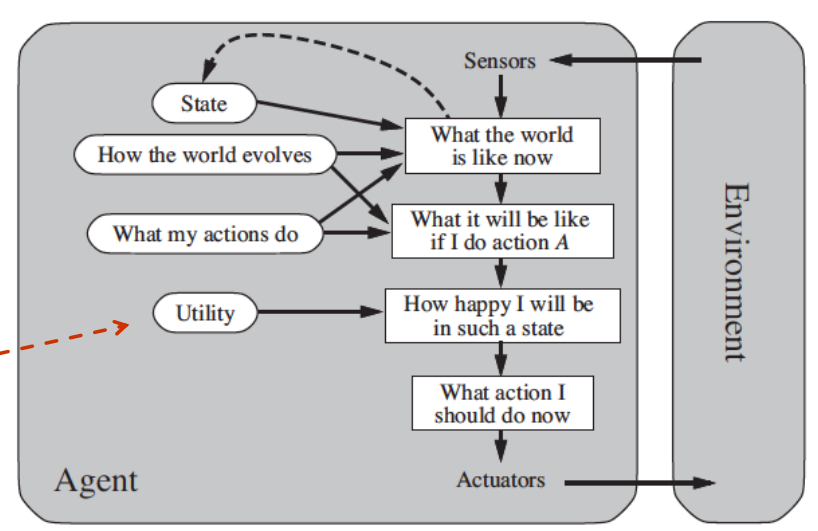
\includegraphics[width=\linewidth]{6.png}

\textbf{Obiettivi alternativi} (o più modi per raggiungerlo) l'agente decide verso quali di questi muoversi, necessita di una funzione di \textit{utilità} che associa ad uno stato obiettivo un numero reale. La funzione di utilità tiene conto anche della probabilità di successo: \textit{utilità attesa}.

\subsection{Agenti che apprendono}

\begin{figure}
    \centering
    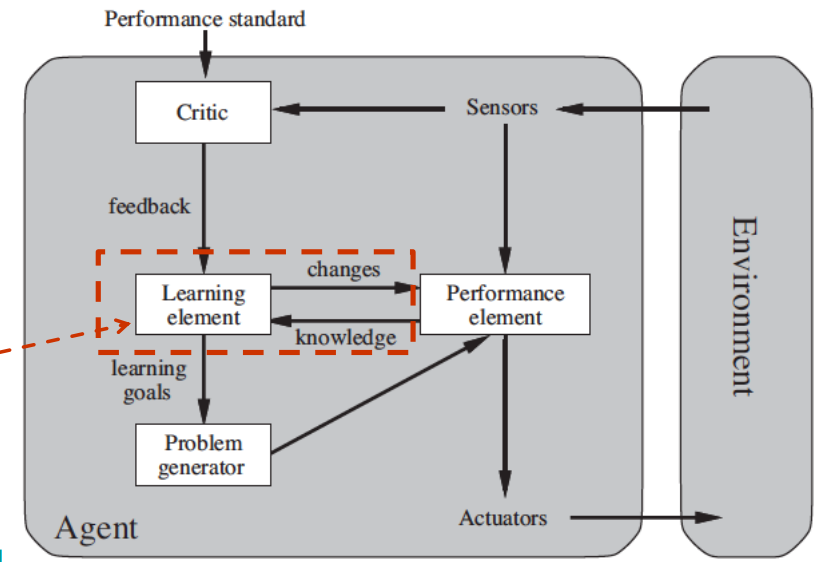
\includegraphics[width =\linewidth]{9.png}
    \caption{Agenti che apprendono}
\end{figure}
\begin{itemize}
    \item Componente di apprendimento: produce cambiamenti al programma agente, apprendendo dall'ambiente
    \item Elemento esecutivo
    \item Elemento critico
    \item Generatore di problemi
\end{itemize}

\subsubsection{Tipi di rappresentazione}

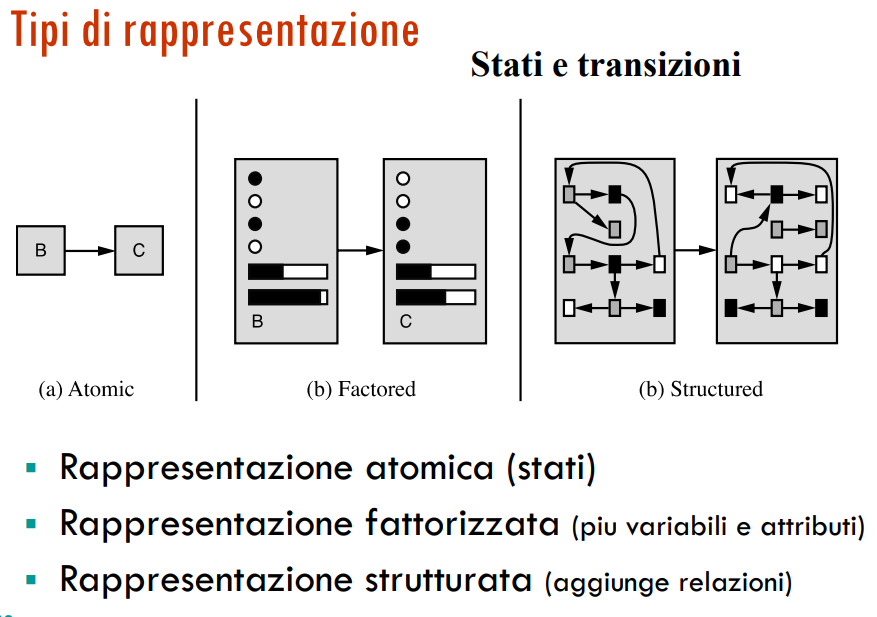
\includegraphics[width=\linewidth]{7.png}

\section{Agenti risolutori di problemi}
Adottano il paradigma della risoluzione di problemi come ricerca in uno spazio di stati (problem solving). Agenti con modello che adottano una rappresentazione atomica dello stato. Sono particolari agenti con obiettivo che pianificano l'intera sequenza di mosse prima di agire

\subsubsection{Processo di risoluzione}

\textbf{Passi da seguire:}
\begin{enumerate}
    \item Determinazione obiettivo (un insieme di stati in cui l'obiettivo è soddisfatto)
    \item Formulazione del problema \qquad \textit{Design (qui ancora umano)}
    \begin{itemize}
        \item rappresentazione degli stati
        \item rappresentazione delle azioni
    \end{itemize}
    \item Determinazione della soluzione mediante \textbf{ricerca} (un piano)
    \item Esecuzione del piano \qquad \textit{Qui soluzione algoritmica}
\end{enumerate}

Assunzioni
\begin{itemize}
    \item Ambiente statico
    \item Osservabile
    \item Discreto
    \item Deterministico
\end{itemize}

\subsubsection{Formulazione del problema}
Un problema può essere definito formalmente mediante cinque componenti:
\begin{enumerate}
    \item Stato iniziale
    \item Azioni possibili in \textit{s}: Azioni(\textit{s})
    \item Modello di transizione:
    \newline Risultato: \textit{stato x azione} $\rightarrow$ \textit{stato}
    \newline Risultato(s,a) = s', uno stato \textbf{successore}
    \newline 1, 2 e 3 definiscono implicitamente lo \textbf{spazio degli stati}
    \item Test obiettivo:
    \begin{itemize}
        \item Un insieme di stati obiettivo
        \item Goal-Test: stato $\rightarrow${\textit{true, false}}
    \end{itemize}
    \item Costo del cammino:
    \begin{itemize}
        \item somma dei costi delle azioni (costo dei passi)
        \item costo di passo: $c(s, a, s')$
        \item Il costo di un'azione/passo non è mai negativo
    \end{itemize}
\end{enumerate}

\section{Algoritmi di ricerca}
Gli algoritmi di ricerca prendono in input un problema e restituiscono un \textbf{cammino soluzione}
\subsection{Problema itinerario}
\begin{figure}
    \centering
    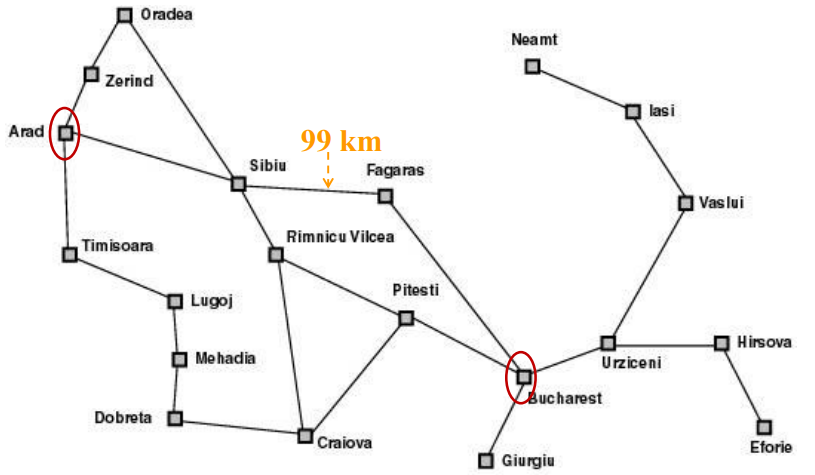
\includegraphics[width=\linewidth]{10.png}
    \caption{caso: trovare il percorso più breve da una città di partenza a una di arrivo}
    \label{fig:my_label}
\end{figure}
\subsubsection{Formulazione}
Stati: le città
\begin{enumerate}
    \item Stato iniziale: città di partenza $In(Arad)$
    \item Azioni: spostarsi su una città vicina collegata $Azioni(In(Arad)) = {Go(Sibiu), Go(Zerind) ...}$
    \item Modello di transizione $Risultato(In(Arad), Go(Sibiu)) = In(Sibiu)$
    \item Test Obiettivo: ${In(Bucarest)}$
    \item Costo del cammino: somma delle lunghezze delle strade
\end{enumerate}

Lo spazio degli stati coincide con la rete di collegamenti tra città

\textbf{Misura delle prestazioni}
\newline Costo totale = costo della ricerca + costo del cammino soluzione

\subsubsection{Ricerca della soluzione}
Generazione di un \textbf{albero di ricerca} sovrapposto allo \textbf{spazio degli stati}
\begin{figure}
    \centering
    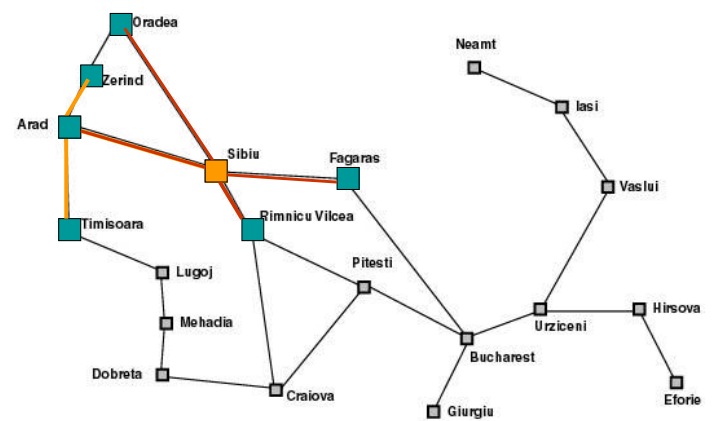
\includegraphics[width = \linewidth]{11.png}
    \caption{albero di ricerca sullo spazio degli stati}
\end{figure}
\textbf{Ricerca}: approfondire un'opzione, da parte le altre e riprenderle se non trova soluzione
\begin{figure}
    \centering
    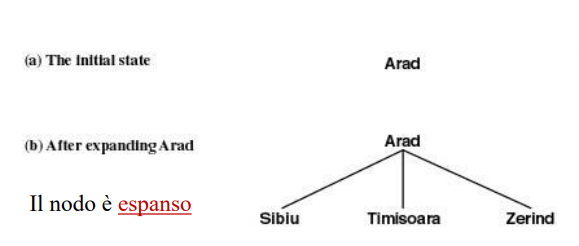
\includegraphics{12.png}
    \caption{Stato iniziale e nodo espanso}
\end{figure}
\subsection{Ricerca ad albero}
\begin{algorithm}
\caption{Ricerca ad albero}
\begin{center}
    \textbf{function} Ricerca-Albero (\textit{problema})\newline
    \textbf{returns} soluzione oppure \textbf{fallimento}\newline
    Inizializza la frontiera con stato iniziale del problema\newline
    \textbf{loop do}\newline
    \textbf{if} \textit{la frontiera è vuota} \textbf{then return fallimento}\newline
    \textit{Scegli un nodo foglia da espandere e rimuovilo dalla frontiera}\newline
    \textbf{if} \textit{il nodo contiene uno stato obiettivo}\newline
    \textbf{then return} \textit{la soluzione corrispondente}\newline
    \textit{Espandi il nodo e aggiungi i successori alla frontiera}
    
\end{center}
\end{algorithm}
\subsection{I nodi dell'albero di ricerca}
Un nodo n è una struttura dati con 4 componenti
\begin{itemize}
    \item Stato: $n.stato$
    \item Nodo padre: $n.padre$
    \item Azione effettuata per generarlo: $n.azione$
    \item Costo del cammino dal nodo iniziale al nodo $n.costo-cammino$ indicata come $g(n) (=padre.costo-cammino+costo-passo\,ultimo$
\end{itemize}
\subsection{Struttura dati per la frontiera}
\textbf{Frontiera}: Lista dei nodi in attesa di essere espandi (foglie dell'albero di ricerca). E' implementata come una cosa con operazioni (empty, POP, Inert)
\subsubsection{Strategie di ricerca}
\begin{itemize}
    \item FIFO $\rightarrow$ BF(Breadth-first): viene estratto l'elemento più vecchio
    \item LIFO $\rightarrow$ DF(Depht-first): viene estratto il più recentemente inserito
    \item Coda con priorità $\rightarrow$ UC: viene estratto quello con priorità più alta in base a una funzione di ordinamento, si riordina ad ogni inserimento di nodi.
\end{itemize}
\subsubsection{Valutazione di una strategia}
\begin{itemize}
    \item Completezza: se la soluzione esiste viene trovata
    \item Ottimalità (ammissibilità): trova la soluzione migliore, con costo minore
    \item Complessità in tempo
    \item Complessità in spazio
    
\end{itemize}

\subsection{Direzione della ricerca}
\textbf{Ricerca in avanti}: (o guidata dai dati) si esplora lo spazio di ricerca dallo stato iniziale allo stato obiettivo
\newline\textbf{Ricerca all'indietro}: (o guidata dall'obiettivo) si esplora lo spazio di ricerca a partire da uno stato goal e riconducendosi a sotto-goal fino a trovare uno stato iniziale.


\section{Ricerca euristica}
La ricerca esaustiva è difficilmente applicabile in problemi di complessità esponenziale. Vogliamo usare la conoscenza euristica per fare scelte "oculate" (conoscenza del problema ed esperienza).
La conoscenza euristica consente di trovare una buona soluzione in tempi accettabili

\subsection{Funzioni di valutazione euristica}
Conoscenza del problema data tramite una \textit{funzione di valutazione f} che include \textit{h} detta funzione di valutazione euristica
\newline $h : n \rightarrow R$
\newline La funzione si applica al nodo ma dipende solo dallo stato (n.Stato)
\begin{figure}
    \begin{equation}
        f(n) = g(n) + h(n)
    \end{equation}
\caption{dove g(n) è il costo del cammino visto con UC}
\end{figure}
%manca descrizione

\subsection{Algoritmo di ricerca Best-First}
Con lo stesso algoritmo di UC, ma con uso di $f$ (stima di costo) per la coda con priorità. La scelta di $f$ determina la strategia di ricerca.

A ogni passo si sceglie il nodo sulla frontiera per cui il valore della $f$ è migliore. In caso di un'euristica che stima la distanza della soluzione migliore significa minore $f<h$, nel caso \textbf{greedy best-first} si usa $f=h$

\subsection{Algoritmo A}
Un algoritmo A è un algoritmo Best First con una funzione di valutazione dello stato del tipo
\begin{equation}
    f(n) = g(n) + h(n),\quad con\,h(n) \geq 0 \,\, e \,\, h(goal) = 0
\end{equation}
\begin{center}
    \begin{itemize}
        \item $g(h)$ è il costo del cammino percorso per raggiungere $n$
        \item $h(n)$ una stima del costo per raggiungere da $n$ un nodo goal
    \end{itemize}
\end{center}

\subsection{Algoritmo A*}
Funzione di valutazione ideale
\begin{equation}
    f\text{*}(n) = g\text{*}(n) + h\text{*}(n)
\end{equation}
\begin{center}
    $g\text{*}(n)$ costo del cammino minimo da radice $n$\newline
    $h\text{*}(n)$ costo del cammino minimo da $n$ a goal\newline
    $f\text{*}(n)$ costo del cammino minimo da radice a goal, attraverso $n$
\end{center}
\subsubsection{Algoritmo A*: definizione}

\begin{definizione}[Euristica ammissibile]
%\begin{center}
$\forall n.h(n) \leq h\text{*}(n)$ \quad $h$ è una sottostima
%\end{center} 
\end{definizione}
\begin{center} \textit{(es. l'euristica della distanza in linea d'aria)}\end{center}
\begin{definizione}[Algoritmo A*]
Un algoritmo A in cui $h$ è una funzione euristica ammissibile
\end{definizione}
\begin{theorem}
Gli algoritmi A* sono \textit{ottimali}
\end{theorem}
\begin{corollary}
BF$^{(+)}$ e UC sono ottimali $(h(n)=0$
\end{corollary}

\section{Ricerca Locale}
Gli algoritmi visti esplorano gli spazi di ricerca alla ricerca di un goal e restituiscono un \textbf{cammino soluzione}. A volte lo stato goal è la soluzione del problema. 

Gli algoritmi di ricerca locale sono adatti per problemi in cui:
\begin{itemize}
    \item La sequenza di azioni non è importante; quello che conta è unicamente lo stato goal
    \item Tutti gli elementi della soluzione sono nello stato, ma alcuni vincolo sono violati
\end{itemize}
\subsection{Proprietà}
\begin{itemize}
    \item Non sono sistematici
    \item Tengono traccia solo del nodo corrente e si spostano su nodi adiacenti
    \item Non tengono traccia dei cammini
    \item Efficienti in occupazione di memoria
    \item Possono trovare soluzioni ragionevoli anche in spazi molto grandi e infiniti (spazi continui)
    \item Utili per risolvere problemi di ottimizzazione
    \begin{itemize}
        \item Lo stato migliore secondo una \textit{funzione obiettivo}
        \item Lo stato di \textit{costo minore}
        \item \textit{es: training di un modello di machine learning}
    \end{itemize}
\end{itemize}
\newpage
\subsection{Panorama dello spazio degli stati}
Uno stato ha una posizione sulla superficie e una altezza che corrisponde al valore della f. di valutazione (f. obiettivo). Un algoritmo provoca un movimento sulla superficie. 
Avvallamento più basso $\rightarrow$ costo minimo o picco più alto $\rightarrow$ max di un obiettivo

\begin{figure}[H]
    \begin{center}
    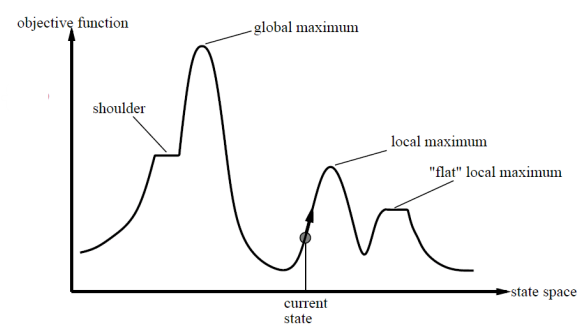
\includegraphics[width = \linewidth]{13.png}
    \caption{f euristica di costo della funzione obiettivo (non del cammino)}
    \end{center}
\end{figure}
\newpage
\subsection{Ricerca in salita (Hill Climbing)}
Ricerca locale \textbf{greedy}. Vengono generati i successori e valutati; viene scelto un nodo che migliora la valutazione dello stato attuale \textit{(non si tiene traccia degli altri)} 
\begin{itemize}
    \item Il migliore $\rightarrow$ \textit{\textbf{Hill climbing a salita rapida/ripida}}
    \item Uno a caso (tra quelli che salgono) $\rightarrow$ \textit{\textbf{Hill climbing stocastico}}
    \item Il primo $\rightarrow$ \textbf{\textit{Hill climbing con prima scelta}}
\end{itemize}
\begin{center} Se non ci sono stati successori migliori, l'algoritmo termina con fallimento\end{center}

\begin{algorithm}[H]
\caption{Algoritmo Hill climbing - steepest ascent}
  
        \textbf{function} Hill-climbing (\textit{problema})\newline
        \null\quad \textbf{returns} uno stato che è un massimo locale\newline
        \null\quad \textit{nodo-corrente} = CreaNodo(\textit{problema.}Stato iniziale)\newline
        \null\quad \textbf{loop do}\newline
        \null\qquad \textit{vicino} = il successori di \textit{nodo-corrente} di valore più alto\newline
        \null\qquad \textbf{if} \textit{vicino}.Valore $\leq$ \textit{nodo-corrente}.Valore \textbf{then} \textbf{return} \textit{nodo-corrente}.Stato //\textit{interrompe la ricerca}\newline
        \null\qquad \textit{nodo-corrente} = vicino //altrimenti, se vicino è migliore, continua
    
\end{algorithm}

\begin{center}
    Si prosegue solo se il vicino (più alto) è migliore dello stato corrente $\rightarrow$ se tutti i vicino sono peggiori si ferma.
    
    Non c'è frontiera a cui ritornare, si tiene un solo stato
    
    Tempo: nuemro cicli variabile in base al punto di partenza
\end{center}
\end{document}
